	
	Dans un repère orthonormé, on considère le point $A(-3 ; 5)$ et la droite $(d)$ dont une équation cartésienne est $-x + 3y + 2 = 0$.
	
	\textbf{Question 1}
	
Avec l'équation de droite, on vérifie que les points $B(2; 0)$ et $C(-4; -2)$ appartenant à la droite $(d)$.

\begin{center}




	
	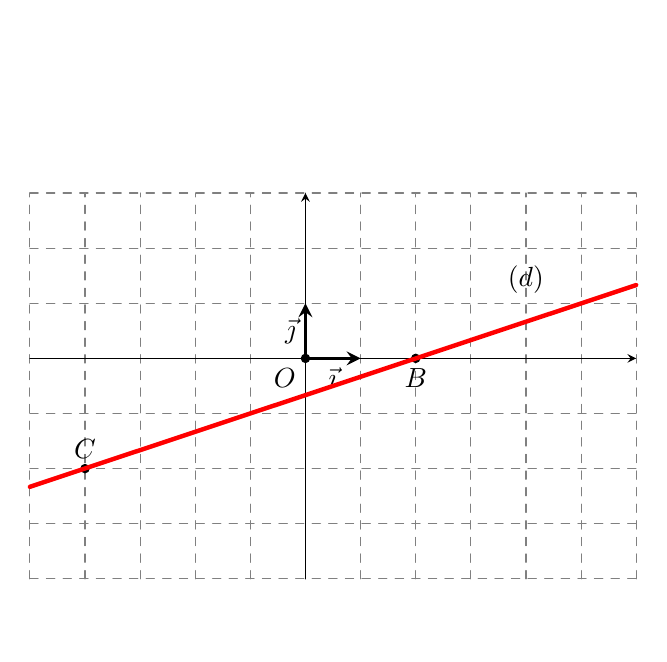
\begin{tikzpicture}[line cap=round,line join=round,>=stealth,x=.7cm,y=.7cm]
		% Grille
		\draw[step=1.0,gray, thin, dashed] (-5,-4) grid (6,3);
		
		% Axes
		\draw[->,color=black] (-5,0) -- (6,0);  % Axe des abscisses
		\draw[->,color=black] (0,-4) -- (0,3);  % Axe des ordonnées
		
		% Origine
		\draw [fill=black] (0,0) circle (1.5pt);
		\draw[color=black] (0,0) node [anchor=north east]{$O$};
		
		% Vecteurs de base
		\draw [->,line width=1.2pt,color=black] (0,0) -- (0,1);  % Vecteur j
		\draw [->,line width=1.2pt,color=black] (0,0) -- (1,0);  % Vecteur i
		
		% Labels des vecteurs
		\draw [color=black](0.5,0) node[anchor=north] {$\vec{\imath}$};  % Vecteur i
		\draw [color=black](0,0.5) node[anchor=east] {$\vec{\jmath}$};   % Vecteur j
		
		\draw [fill=black] (2,0) circle (1.5pt);
		\draw [fill=black] (2,0) node [anchor=north]{$B$};
			\draw [fill=black] (-4,-2) circle (1.5pt);
		\draw [fill=black] (-4,-2) node [anchor=south]{$C$};
		\draw[red,ultra thick](-5,-2.33)--(6,1.33);
			\draw [fill=black] (4,1) node [anchor=south]{$(d)$};
		% Limites du dessin
		\clip(-5,-5) rectangle (6,6);
	\end{tikzpicture}
	


\end{center}

	
	\textbf{Question 2}
	
	Un vecteur directeur de la droite $(d)$ a pour coordonnées $\begin{pmatrix}
		3\\
		1
	\end{pmatrix}$, donc un vecteur normal est par exemple $\vec{n}\begin{pmatrix}
	1\\
	-3
	\end{pmatrix}$. 
	
	\textbf{Question 3}
	
	Si $\delta$ est la perpendiculaire à $(d)$ passant par $A$, on a :
	\[
	M(x; y) \in \delta \iff \overrightarrow{AM} \text{ et } \vec{n} \text{ sont colinéaires, soit } -3(x + 3) = 1(y - 5).
	\]
	Cela donne l'équation :
	\[
	3x - y + 14 = 0.
	\]
	
\textbf{Question 4}

Le projeté orthogonal de $A$ sur la droite $(d)$ est le point commun de $(d)$ et $\delta$. On résout le système d'équations :
\[
\begin{cases}
	-x + 3y + 2 = 0 \\
	3x - y + 14 = 0
\end{cases}
\]
Cela donne :
\begin{align*}
	x &= 3y + 2 \\
	3(3y + 2) - y + 14 &= 0 \\
	9y + 6 - y + 14 &= 0 \\
	8y &= -20 \\
	y &= -\dfrac{5}{2}.
\end{align*}

On trouve $x = 3y + 2 = 3 \times \left(-\dfrac{5}{2}\right) + 2 = -\dfrac{11}{2}$.\\
 Le projeté orthogonal est donc le point $H\left(-\dfrac{11}{2}, -\dfrac{5}{2}\right)$.

\textbf{Question 5}

La distance entre le point $A$ et la droite $(d)$ est égale à $AH$. On calcule :
\begin{align*}
	AH^2 &= \left(-\dfrac{11}{2} + 3\right)^2 + \left(-\dfrac{5}{2} - 5\right)^2 \\
	&= \left(-\dfrac{5}{2}\right)^2 + \left(-\dfrac{15}{2}\right)^2 \\
	&= \dfrac{25}{4} + \dfrac{225}{4} \\
	&= \dfrac{250}{4}, \quad \text{d'où} \quad AH = \dfrac{\sqrt{250}}{2}.
\end{align*}

